%!TEX root = ../../../adrien_gomar_phd.tex

Both the mono- and multi-frequential harmonic balance
approaches have been on a linear equation. In the following
section, the multi-frequential harmonic balance developed and
implemented by \citet{ThesisGuedeney} into the \emph{elsA}~\cite{Cambier2013}
CFD code is assessed within a non-linear framework, namely the
Navier--Stokes equations.

\subsection{Presentation of the case}
\label{sec:channel_flow_problem}

The second case consists of a 2D channel 
with a constant left injection at 
a transonic Mach number ($M_0=0.7$)
supplemented with a time-varying unsteady back pressure.
As the pressure is oscillating at the outlet, the imposed unsteady pressure
fluctuations travel within the flow at the velocity 
$u + c$ and $u - c$, where $u$ denotes 
the local flow velocity and $c$ the speed of sound.
Since the pressure waves are generated at the outlet, only
the $u-c$ waves are seen, resulting in pressure waves propagating
upstream of the channel. The axial length of the channel is $L_x = 100$~m
and the transversal one is $L_y = 1$~m.
Figure~\ref{fig:canal_principle} shows a sketch
of the considered channel flow problem.
\begin{figure}[htp]
  \centering
  \includegraphics*[width=0.65\textwidth]{channel_sketch.pdf}
  \caption{Sketch of the channel flow problem.}
  \label{fig:canal_principle}
\end{figure}

\citet{Merkle1987} give an analytical solution
for incompressible flows with small pressure fluctuations, assuming
thus a linear unsteady flow.
However, this channel flow problem is set up to highlight the properties
of the harmonic balance in a non-linear framework which is not
the hypothesis of \citet{Merkle1987}. Nevertheless, to give confidence
in our forthcoming results for this model problem,
this last will be validated below against a classical time-marching scheme
in Sec.~\ref{sec:channel_multifreq}.

\subsection{Numerical setup}

% mesh presentation
The mesh consists of 997~points along the axial direction and 9~in the
transverse one, which corresponds to equal spacings in both
directions. 

% boundary conditions
The boundary conditions are: (i)~a constant injection condition for the inlet
where the total pressure $p_{i_0}$ and enthalpy $h_{i_0}$ are set,
(ii)~symmetric conditions for the upper and lower bounds as the flow
is assumed to be symmetric in the transverse direction, and (iii)~a
fluctuating static pressure imposed at the outlet
\begin{equation}
  p_{s_1}(t) = \overline{p}_{s_1} \left[1 + a_1 \sin(2 \pi f_1 t) +
    a_2 \sin(2 \pi f_2 t) \right],
  \label{eq:outlet_canal}
\end{equation}
where $\overline{p}_{s_1}$ is the temporal average static pressure, $a_n$ the
amplitude of the $n$\textsuperscript{th} mode and $f_n$ its
frequency. Only two modes ($f_1$, $f_2$) are injected
but due to the non-linearity of the Navier--Stokes equations,
new frequency combinations rise.
The mean velocity of the flow is imposed through a
static pressure condition $\overline{p}_{s_1}$ at the outlet
\begin{equation}
    \overline{p}_{s_1} = \frac{p_{i_0}}{\left(1 + 
    \frac{\gamma - 1}{2} M_{0}^2 \right) ^ {\frac{\gamma}{ \gamma - 1}}} ,
\end{equation}
the mean velocity is thus set by imposing the
inlet target mean Mach number value $M_{0}$.
We assume here that the flow is isentropic as no
geometrical object disturbes the flow field.

% solver
The \textit{elsA}~\cite{Cambier2013} CFD code developed by ONERA
is used to solve this channel flow problem. In fact, 
the aim of this model problem is 
to use the same
solver as the one used in the application part of this
thesis so that the results shown here can be directly
transposed later on.
This code solves the RANS equations using a cell-centered
approach on multi-blocks structured meshes.
Several time-integration schemes
are available, in particular the Dual Time-Stepping~\cite{Jameson1981} (DTS)
as well as the time-domain harmonic 
balance method implemented by \citet{JSicot2008} for the mono-frequential
formulation and extended by \citet{JGuedeney2013} to multi-frequential flows. 


% numerical schemes
The present configuration is turbulent as the Reynolds number based on the
inlet flow velocity and the axial length of the channel is about $R_e
\approx 2.0 \times 10^9$. To this aim, turbulence is modeled using the
one-equation model of \citet{Spalart1992}.
Roe's scheme~\cite{Roe1981} along with a third-order MUSCL extrapolation 
is used for the spatial discretization of
the convective fluxes. An implicit backward Euler scheme is used
to march the HB equations in pseudo-time.

\subsection{Validation of the multi-frequential approach}
\label{sec:channel_multifreq}

We propose
now to validate the channel flow problem within 
the multi-frequential harmonic balance framework
in order to have confidence in the forthcoming results that
will use this approach.
To do so, two non-harmonically related
frequencies are chosen as input for the outlet boundary condition:
$f_1 = 3$~Hz and $f_2 = 17$~Hz.

The classical DTS time-marching scheme is taken for comparison.
Convergence in time discretization is obtained after 20~periods using
160~instants per almost-period. Since the frequencies are integers and
coprime, the period is $T=1$~s.  Iterative convergence for the
inner loop is considered achieved when the normalized residuals drop
by $10^{-2}$ within a maximum of 50~sub-iterations.

The results obtained with the DTS scheme are compared to the HB
results for pressure waves amplitudes of $a = a_1 = a_2 = 0.001$
(see Eq.~\eqref{eq:outlet_canal}). The
transient of the DTS computation is shown in
Figure~\ref{fig:canal2_transient}, illustrating the wave propagation
with a slight attenuation of the high-frequency waves.
\begin{figure}[htp]
  \centering
  \includegraphics*[width=.5\linewidth]{CANAL2_TRANSIENT_PPT.pdf}
  \caption{DTS computation: transient propagation of the pressure waves.}
  \label{fig:canal2_transient}
\end{figure}

Due to the non-linearity of the Navier--Stokes equations, the two frequencies
$f_1$ and $f_2$ give rise to linear combinations of them.
Therefore, the results are analyzed for frequencies $1<f< 40~\textrm{Hz}$ and the
dominant frequencies (the one that have the highest amplitudes) are
set for the HB computation.  To do so, pressure signals are probed
upstream, in the middle and downstream of the channel at
$x=[25~\textrm{m}, 50~\textrm{m}, 75~\textrm{m}]$ and $y=0.5$~m
respectively.  The spectra of the aforementioned unsteady pressure
signals, obtained with a Fourier Transform are plotted in
Figure~\ref{fig:canal2_dts_fft}.  The labeled frequencies are the
dominant ones, as for each probe, these have a high amplitude. Those
nine frequencies are thus selected as input frequencies for the HB computation.
Actually, this corresponds to a rectangular grid truncation 
(see Sec.~\ref{sec:sm_hb_extension}).
\begin{figure}[htp]
  \centering
  \includegraphics*[width=.5\linewidth]{channel_dts_fft_plus_sketch.pdf}
  \caption{Spectra of the pressure signals.}
  \label{fig:canal2_dts_fft}
\end{figure}

The HB computation using the previously mentioned frequencies is
run and a discrete Fourier transform is computed at several axis positions
in the middle of the channel ($y=0.5$~m). 
This is the same post-processing as done previously to retrieve 
Figure~\ref{fig:canal2_dts_fft}, but for all axial grid points.
Figure~\ref{fig:canal2_validation_hbt_gear_amp_vs_axis}
shows the results for the frequencies that have been set for the 
multi-frequential HB computation.
The overall agreement between the DTS and the HB is fair.  
Some local discrepancies can be
observed upstream for frequencies $f_2 + 3f_1$, $f_2 - f_1$ and $f_2 -
2f_1$. 
\begin{figure}[htp]
  \centering
  \includegraphics*[width=.5\linewidth]{CANAL2_VALIDATION_HBT_GEAR_PPT_AMP_VS_AXIS.pdf}
  \caption{Spatial evolution of the amplitude of the dominant
    frequencies in the channel flow configuration, for $f_1 = 3$~Hz and $f_2 = 17$~Hz.}
  \label{fig:canal2_validation_hbt_gear_amp_vs_axis}
\end{figure}
These are caused by aliasing
but they are minimal regarding the temporal evolution, as
shown in Figure~\ref{fig:canal2_validation_hbt_gear_time_ev}, where the
time evolution of pressure signals is extracted at all probes.  The
difference between the HB and the DTS method is negligible proving
that the present multi-frequential harmonic balance approach is
able to accurately retrieve multi-frequential unsteadinesses.
\begin{figure}[htp]
  \centering 
  \subfigure[probe
  1]{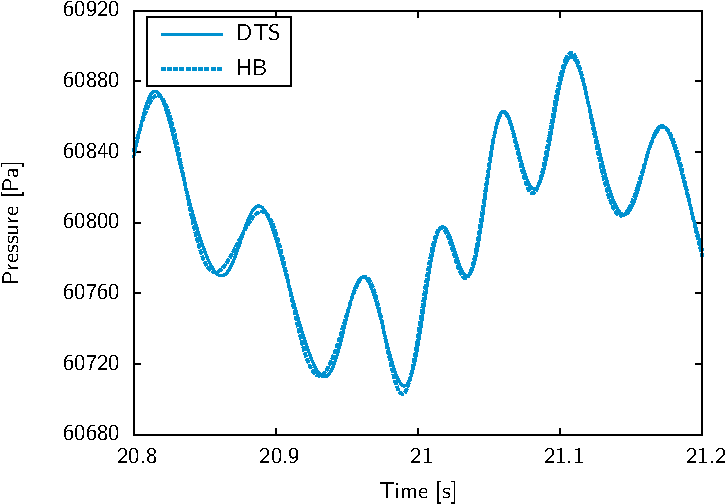
\includegraphics[width=.4\textwidth]{CANAL2_VALIDATION_HBT_GEAR_TIME_EV_PROBE_1_PPT.pdf}}
   \quad\subfigure[probe
   2]{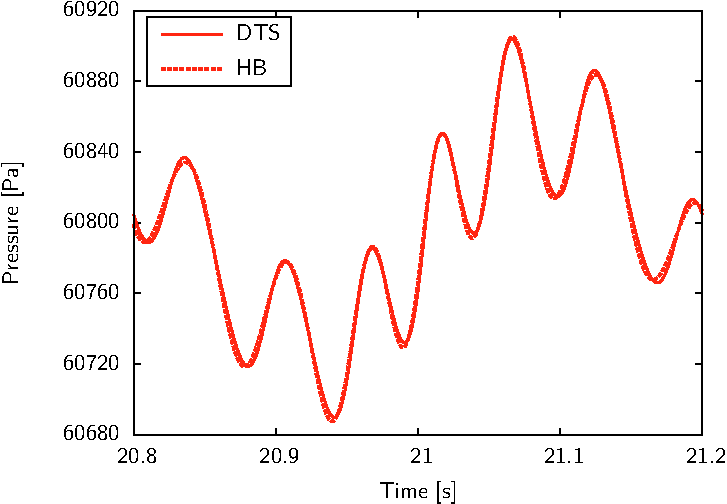
\includegraphics[width=.4\textwidth]{CANAL2_VALIDATION_HBT_GEAR_TIME_EV_PROBE_2_PPT.pdf}}
   \subfigure[probe
   3]{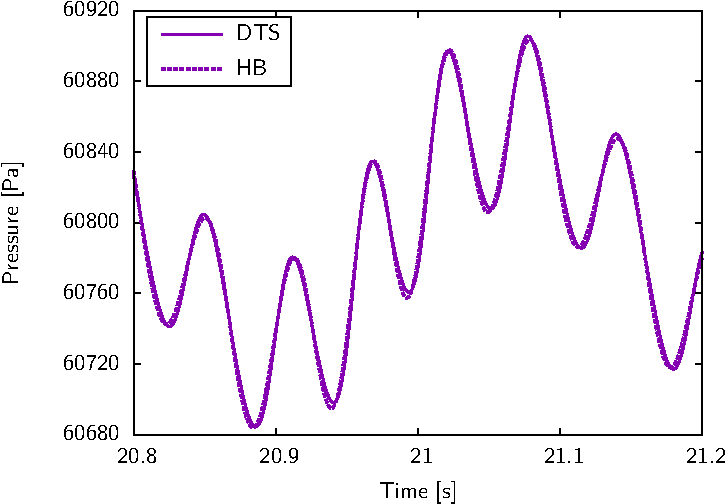
\includegraphics[width=.4\textwidth]{CANAL2_VALIDATION_HBT_GEAR_TIME_EV_PROBE_3_PPT.pdf}}
  \caption{Unsteady pressure signals at different axial positions.}
  \label{fig:canal2_validation_hbt_gear_time_ev}
\end{figure}
